% Options for packages loaded elsewhere
\PassOptionsToPackage{unicode}{hyperref}
\PassOptionsToPackage{hyphens}{url}
%
\documentclass[
  ,man,floatsintext]{apa6}
\usepackage{amsmath,amssymb}
\usepackage{lmodern}
\usepackage{iftex}
\ifPDFTeX
  \usepackage[T1]{fontenc}
  \usepackage[utf8]{inputenc}
  \usepackage{textcomp} % provide euro and other symbols
\else % if luatex or xetex
  \usepackage{unicode-math}
  \defaultfontfeatures{Scale=MatchLowercase}
  \defaultfontfeatures[\rmfamily]{Ligatures=TeX,Scale=1}
\fi
% Use upquote if available, for straight quotes in verbatim environments
\IfFileExists{upquote.sty}{\usepackage{upquote}}{}
\IfFileExists{microtype.sty}{% use microtype if available
  \usepackage[]{microtype}
  \UseMicrotypeSet[protrusion]{basicmath} % disable protrusion for tt fonts
}{}
\makeatletter
\@ifundefined{KOMAClassName}{% if non-KOMA class
  \IfFileExists{parskip.sty}{%
    \usepackage{parskip}
  }{% else
    \setlength{\parindent}{0pt}
    \setlength{\parskip}{6pt plus 2pt minus 1pt}}
}{% if KOMA class
  \KOMAoptions{parskip=half}}
\makeatother
\usepackage{xcolor}
\usepackage{graphicx}
\makeatletter
\def\maxwidth{\ifdim\Gin@nat@width>\linewidth\linewidth\else\Gin@nat@width\fi}
\def\maxheight{\ifdim\Gin@nat@height>\textheight\textheight\else\Gin@nat@height\fi}
\makeatother
% Scale images if necessary, so that they will not overflow the page
% margins by default, and it is still possible to overwrite the defaults
% using explicit options in \includegraphics[width, height, ...]{}
\setkeys{Gin}{width=\maxwidth,height=\maxheight,keepaspectratio}
% Set default figure placement to htbp
\makeatletter
\def\fps@figure{htbp}
\makeatother
\setlength{\emergencystretch}{3em} % prevent overfull lines
\providecommand{\tightlist}{%
  \setlength{\itemsep}{0pt}\setlength{\parskip}{0pt}}
\setcounter{secnumdepth}{-\maxdimen} % remove section numbering
% Make \paragraph and \subparagraph free-standing
\ifx\paragraph\undefined\else
  \let\oldparagraph\paragraph
  \renewcommand{\paragraph}[1]{\oldparagraph{#1}\mbox{}}
\fi
\ifx\subparagraph\undefined\else
  \let\oldsubparagraph\subparagraph
  \renewcommand{\subparagraph}[1]{\oldsubparagraph{#1}\mbox{}}
\fi
\ifLuaTeX
\usepackage[bidi=basic]{babel}
\else
\usepackage[bidi=default]{babel}
\fi
\babelprovide[main,import]{english}
% get rid of language-specific shorthands (see #6817):
\let\LanguageShortHands\languageshorthands
\def\languageshorthands#1{}
% Manuscript styling
\usepackage{upgreek}
\captionsetup{font=singlespacing,justification=justified}

% Table formatting
\usepackage{longtable}
\usepackage{lscape}
% \usepackage[counterclockwise]{rotating}   % Landscape page setup for large tables
\usepackage{multirow}		% Table styling
\usepackage{tabularx}		% Control Column width
\usepackage[flushleft]{threeparttable}	% Allows for three part tables with a specified notes section
\usepackage{threeparttablex}            % Lets threeparttable work with longtable

% Create new environments so endfloat can handle them
% \newenvironment{ltable}
%   {\begin{landscape}\centering\begin{threeparttable}}
%   {\end{threeparttable}\end{landscape}}
\newenvironment{lltable}{\begin{landscape}\centering\begin{ThreePartTable}}{\end{ThreePartTable}\end{landscape}}

% Enables adjusting longtable caption width to table width
% Solution found at http://golatex.de/longtable-mit-caption-so-breit-wie-die-tabelle-t15767.html
\makeatletter
\newcommand\LastLTentrywidth{1em}
\newlength\longtablewidth
\setlength{\longtablewidth}{1in}
\newcommand{\getlongtablewidth}{\begingroup \ifcsname LT@\roman{LT@tables}\endcsname \global\longtablewidth=0pt \renewcommand{\LT@entry}[2]{\global\advance\longtablewidth by ##2\relax\gdef\LastLTentrywidth{##2}}\@nameuse{LT@\roman{LT@tables}} \fi \endgroup}

% \setlength{\parindent}{0.5in}
% \setlength{\parskip}{0pt plus 0pt minus 0pt}

% Overwrite redefinition of paragraph and subparagraph by the default LaTeX template
% See https://github.com/crsh/papaja/issues/292
\makeatletter
\renewcommand{\paragraph}{\@startsection{paragraph}{4}{\parindent}%
  {0\baselineskip \@plus 0.2ex \@minus 0.2ex}%
  {-1em}%
  {\normalfont\normalsize\bfseries\itshape\typesectitle}}

\renewcommand{\subparagraph}[1]{\@startsection{subparagraph}{5}{1em}%
  {0\baselineskip \@plus 0.2ex \@minus 0.2ex}%
  {-\z@\relax}%
  {\normalfont\normalsize\itshape\hspace{\parindent}{#1}\textit{\addperi}}{\relax}}
\makeatother

% \usepackage{etoolbox}
\makeatletter
\patchcmd{\HyOrg@maketitle}
  {\section{\normalfont\normalsize\abstractname}}
  {\section*{\normalfont\normalsize\abstractname}}
  {}{\typeout{Failed to patch abstract.}}
\patchcmd{\HyOrg@maketitle}
  {\section{\protect\normalfont{\@title}}}
  {\section*{\protect\normalfont{\@title}}}
  {}{\typeout{Failed to patch title.}}
\makeatother

\usepackage{xpatch}
\makeatletter
\xapptocmd\appendix
  {\xapptocmd\section
    {\addcontentsline{toc}{section}{\appendixname\ifoneappendix\else~\theappendix\fi\\: #1}}
    {}{\InnerPatchFailed}%
  }
{}{\PatchFailed}
\usepackage{lineno}

\linenumbers
\usepackage{csquotes}
\usepackage{amsmath}
\usepackage[labelformat=empty]{caption}
\usepackage{caption}
\usepackage[extra]{tipa}
\renewcommand{\topfraction}{1}
\renewcommand{\bottomfraction}{1}
\renewcommand{\textfraction}{.1}
\renewcommand{\floatpagefraction}{1}
\setcounter{topnumber}{9}
\setcounter{bottomnumber}{9}
\setcounter{totalnumber}{20}
\setcounter{dbltopnumber}{9}
\renewcommand{\thefigure}{S\arabic{figure}}
\ifLuaTeX
  \usepackage{selnolig}  % disable illegal ligatures
\fi
\IfFileExists{bookmark.sty}{\usepackage{bookmark}}{\usepackage{hyperref}}
\IfFileExists{xurl.sty}{\usepackage{xurl}}{} % add URL line breaks if available
\urlstyle{same} % disable monospaced font for URLs
\hypersetup{
  pdftitle={Supplemental Materials},
  pdfauthor={Lori Mitchell1, Rachel Ka-Ying Tsui1, \& Krista Byers-Heinlein1},
  pdflang={en-EN},
  hidelinks,
  pdfcreator={LaTeX via pandoc}}

\title{Supplemental Materials}
\author{Lori Mitchell\textsuperscript{1}, Rachel Ka-Ying Tsui\textsuperscript{1}, \& Krista Byers-Heinlein\textsuperscript{1}}
\date{}


\shorttitle{Cognate advantage in bilingual infants}

\authornote{

Correspondence concerning this article should be addressed to Rachel Ka-Ying Tsui, Department of Psychology, 7141 Sherbrooke St.~West, Montreal, QC, Canada, H2T1V2. Rachel Ka-Ying Tsui is now at Laboratory for Language Development, RIKEN Center for Brain Science, 2-1 Hirosawa, Wako-shi, Saitama, Japan, 351-0198. E-mail: \href{mailto:rachelkytsui@gmail.com}{\nolinkurl{rachelkytsui@gmail.com}}

}

\affiliation{\vspace{0.5cm}\textsuperscript{1} Concordia University}

\begin{document}
\maketitle

\captionsetup[table]{labelformat=empty}

Using the more stringent 25\%-75\% language exposure criterion, we further eliminated a total of 9 bilingual infants who had a wider language exposure range. This left us with data from 41 participants (23 girls; mean starting age = 18 months, \(SD\) = 1.17, range = 16.20 -- 20.40; mean ending age = 21.84 months, \(SD\) = 3.43, range = 16.30 -- 27.14), with 180 English CDI administrations and 176 French CDI administration. As in the main analysis, we retained only those administrations where both the English and French were completed at the same time point; this gave us 172 completed administrations from 38 infants. Among the 38 infants, 5 infants contributed data at only one time point, and 33 infants contributed data at more than one time point, with participants contributing an average of 4.53 measurements for each language (\(SD\) = 2.63, range = 1 -- 10).

On average, this group of 38 infants were exposed to English 50.90\% of the time (\(SD\) = 10.70, range = 26 -- 74), to French 48.50\% of the time (\(SD\) = 11.20, range = 26 -- 74), and to a third language 0.60\% of the time (\(SD\) = 1.50, range = 0 -- 5). 22 of the bilingual infants were English-dominant (\(M\) = 57.30\% English exposure, \(SD\) = 7.70, range = 49 -- 74), 15 were French-dominant (\(M\) = 59.40\% French exposure, \(SD\) = 6.10, range = 51 -- 74), and 1 reported equal exposure to both English and French. The average maternal education level was 17.32 years (\(SD\) = 2, range = 12 -- 23), and 92.11\% of the mothers had completed a university degree or higher.

\hypertarget{descriptive-measures-of-number-of-words-produced}{%
\subsection{Descriptive Measures of Number of Words Produced}\label{descriptive-measures-of-number-of-words-produced}}

Out of the complete list, bilingual infants on average produced a total of 164 words (\(SD\) = 170.16), with a range of 0 -- 709 words, which constituted 15.28\% of the words on the complete list. Moreover, they produced an average of 44 complete translation equivalent pairs where both the English and French words were produced (\(SD\) = 54.52, range = 0 -- 243), which constituted 8.27\% of the translation equivalent pairs on the complete list.

As for the matched list, bilingual infants produced an average of 53 words (\(SD\) = 64.23, range = 0 -- 248), which constituted 16.49\% of the words on the matched list. On average, bilingual infants produced a total of 14 complete translation equivalent pairs (\(SD\) = 22.52, range = 0 -- 92), which constituted 8.79\% of translation equivalent pairs on the matched list.

\hypertarget{dependent-variable-1-cognate-words-versus-non-cognate-words}{%
\subsection{Dependent Variable 1: Cognate Words Versus Non-Cognate Words}\label{dependent-variable-1-cognate-words-versus-non-cognate-words}}

Following the procedure in the main analysis, we first looked at the total proportion of words infants produced on the relevant list. Our predictor variables were age (in days) and cognate status. Age was continuous and was centered at the mean age of 548.3 days (approximately 18 months) for ease of interpretation. Cognate status was categorical with two levels (cognates versus non-cognates) with non-cognates as the reference level. We ran separate logistic regression models for the complete and matched lists. The initial model specification included a random slope of age and cognate status by participants, which was pruned to a random intercept to achieve model convergence. The final model was:

proportion\_word \textasciitilde{} age * cognate\_status + (1\textbar participant)

\hypertarget{complete-list}{%
\subsubsection{Complete List}\label{complete-list}}

Out of the complete list which contained 262 cognate words (i.e., adding the 131 English cognate words and 131 French cognate words) and 812 non-cognate words (i.e., adding the 406 English non-cognate words and 406 French non-cognate words), bilingual infants produced an average of 56 cognate words (\(SD\) = 48.84, range = 0 -- 204) and 108 non-cognate words (\(SD\) = 121.96, range = 0 -- 505). The proportion of cognate words produced was 0.21 (\(SD\) = 0.19, range = 0 -- 0.78), whereas the proportion of non-cognate words produced was 0.13 (\(SD\) = 0.15, range = 0 -- 0.62). Table S1 shows the coefficient estimates for the model and Figure S1 Panel A visualizes the model. Similar to the results reported in the main analysis, we observed significant main effects of age and cognate status, as well as a significant interaction. Overall, the pattern of results was the same as that of the main analysis.

\hypertarget{matched-list}{%
\subsubsection{Matched List}\label{matched-list}}

Out of the 162 cognate (i.e., adding the 81 English cognate words and 81 French cognate words) and 162 non-cognate words (i.e., adding the 81 English non-cognate words and 81 French non-cognate words) on the matched list, bilingual infants produced an average of 29 cognate words (\(SD\) = 33.82, range = 0 -- 135) and 25 non-cognate words (\(SD\) = 30.62, range = 0 -- 113). The overall mean proportion of cognate words produced was 0.18 of words (\(SD\) = 0.21, range = 0 -- 0.83), whereas the proportion of non-cognate words produced was 0.15 (\(SD\) = 0.19, range = 0 -- 0.70). Table S1 also shows the coefficient estimates for the matched list model and Figure S1 Panel B visualizes the model. There were significant effects of age and cognate status, once again showing that infants produced a greater proportion of cognates than non-cognates on the matched list; there was no interaction between cognate status and age. Again, we observed the same patterns as those reported in the main analysis.

\begin{table}[H]

\begin{center}
\begin{threeparttable}

\caption{\label{tab:Table S1}Table S1. Coefficient estimates from the mixed-effects logistic models predicting proportion of words produced.}

\begin{tabular}{lcccccccc}
\toprule
 & \multicolumn{4}{c}{Complete list} & \multicolumn{4}{c}{Matched list} \\
\cmidrule(r){2-5} \cmidrule(r){6-9}
 & Estimate & $SE$ & $z$ & $p$ & Estimate & $SE$ & $z$ & $p$\\
\midrule
Intercept & -2.58 & 0.17 & -15.10 & <.001 & -2.81 & 0.25 & -11.44 & <.001\\
cognate\_status & 0.76 & 0.02 & 44.28 & <.001 & 0.24 & 0.03 & 7.77 & <.001\\
age\_days & 0.01 & 0.00 & 75.69 & <.001 & 0.01 & 0.00 & 40.64 & <.001\\
cognate\_status * age\_days & 0.00 & 0.00 & -5.76 & <.001 & 0.00 & 0.00 & 0.57 & 0.572\\
\bottomrule
\end{tabular}

\end{threeparttable}
\end{center}

\end{table}

\begin{figure}

{\centering 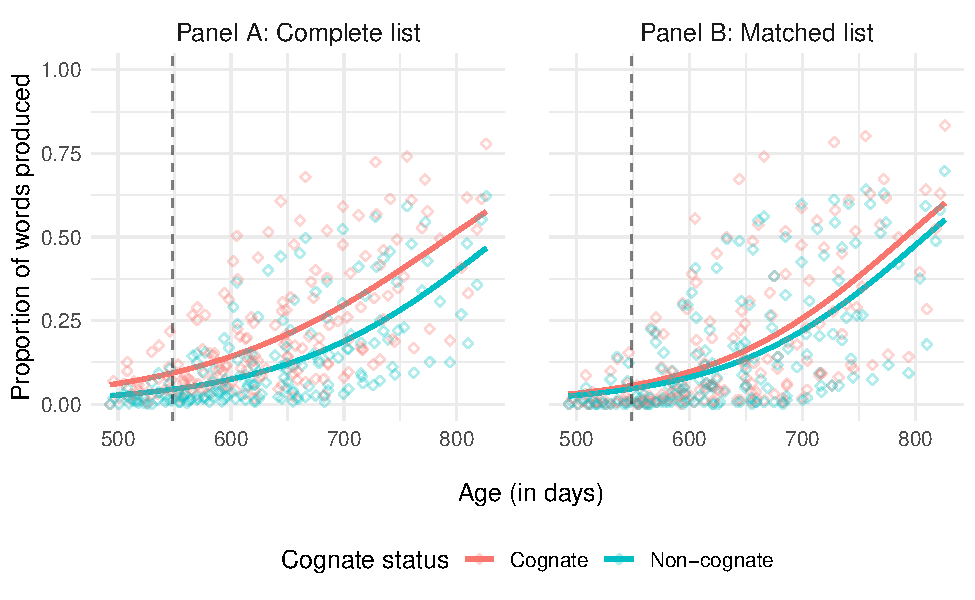
\includegraphics[width=1.2\linewidth]{CogVocab_supplemental_files/figure-latex/FigS1-1} 

}

\caption{Proportion of words produced by age and cognate status, with Panel A representing the complete list and Panel B representing the matched list. Note that the black dashed line represents the mean age of 548.3 days which serves as the reference level for age in our models.}\label{fig:FigS1}
\end{figure}

\hypertarget{dependent-variable-2-cognate-pairs-versus-non-cognate-pairs}{%
\subsection{Dependent Variable 2: Cognate Pairs Versus Non-Cognate Pairs}\label{dependent-variable-2-cognate-pairs-versus-non-cognate-pairs}}

Again, following the procedure reported in the main analysis, the proportion of translation equivalent pairs produced was entered as the dependent variable in the following analysis. Age and cognate status were entered as our predictor variables, with non-cognates set as the reference level, and we ran separate logistic models for the complete and matched lists. The initial model specification, which included a random effect of age and cognate status by participants, had to be reduced for model convergence; therefore, the final model was:

proportion\_pair \textasciitilde{} age * cognate\_status + (1\textbar participant)

\hypertarget{complete-list-1}{%
\subsubsection{Complete List}\label{complete-list-1}}

Out of the complete list which contained 537 translation equivalent pairs (131 cognates and 406 non-cognates), bilingual infants produced an average of 19 cognate pairs (\(SD\) = 19.39, range = 0 -- 82) and 26 non-cognate pairs (\(SD\) = 35.57, range = 0 -- 167). The proportion of cognate pairs produced was 0.14 (\(SD\) = 0.15, range = 0 -- 0.63) whereas the proportion of non-cognate pairs produced was 0.06 (\(SD\) = 0.09, range = 0 -- 0.41). Table S2 shows the coefficient estimates for the model and Figure S2 Panel A visualizes the model. Again, similar to the pattern reported in the main analysis, there were significant effects of age and cognate status and a significant interaction between age and cognate status. Therefore, we observed the same findings as in the main analysis, where overall infants produced a greater proportion of cognates than non-cognates and there is a slightly steeper learning curve for non-cognates than cognates.

\hypertarget{matched-list-1}{%
\subsubsection{Matched List}\label{matched-list-1}}

Out of the 162 translation equivalent pairs, bilingual infants produced an average of 9 cognate pairs (\(SD\) = 13.18, range = 0 -- 58) and 6 non-cognate pairs (\(SD\) = 9.64, range = 0 -- 42). The proportion of cognate pairs produced was 0.11 (\(SD\) = 0.16, range = 0 -- 0.72) and the proportion of non-cognate pairs produced was 0.07 (\(SD\) = 0.12, range = 0 -- 0.52). The coefficient estimates for the matched list model is shown in Table S2, and Figure S2 Panel B visualizes the model. Again, we observed similar pattern of results as those reported in the main analysis, with significant effects of age and cognate status but no significant interaction between age and cognate status.

\begin{table}[tbp]

\begin{center}
\begin{threeparttable}

\caption{\label{tab:Table S2}Table S2. Coefficient estimates from the mixed-effects logistic models predicting proportion of translation equivalent pairs produced.}

\begin{tabular}{lcccccccc}
\toprule
 & \multicolumn{4}{c}{Complete list} & \multicolumn{4}{c}{Matched list} \\
\cmidrule(r){2-5} \cmidrule(r){6-9}
 & Estimate & $SE$ & $z$ & $p$ & Estimate & $SE$ & $z$ & $p$\\
\midrule
Intercept & -3.58 & 0.17 & -20.64 & <.001 & -4.18 & 0.28 & -14.78 & <.001\\
cognate\_status & 1.17 & 0.03 & 36.96 & <.001 & 0.64 & 0.07 & 9.88 & <.001\\
age\_days & 0.01 & 0.00 & 43.62 & <.001 & 0.01 & 0.00 & 24.27 & <.001\\
cognate\_status * age\_days & 0.00 & 0.00 & -5.58 & <.001 & 0.00 & 0.00 & -0.79 & 0.43\\
\bottomrule
\end{tabular}

\end{threeparttable}
\end{center}

\end{table}

\begin{figure}

{\centering 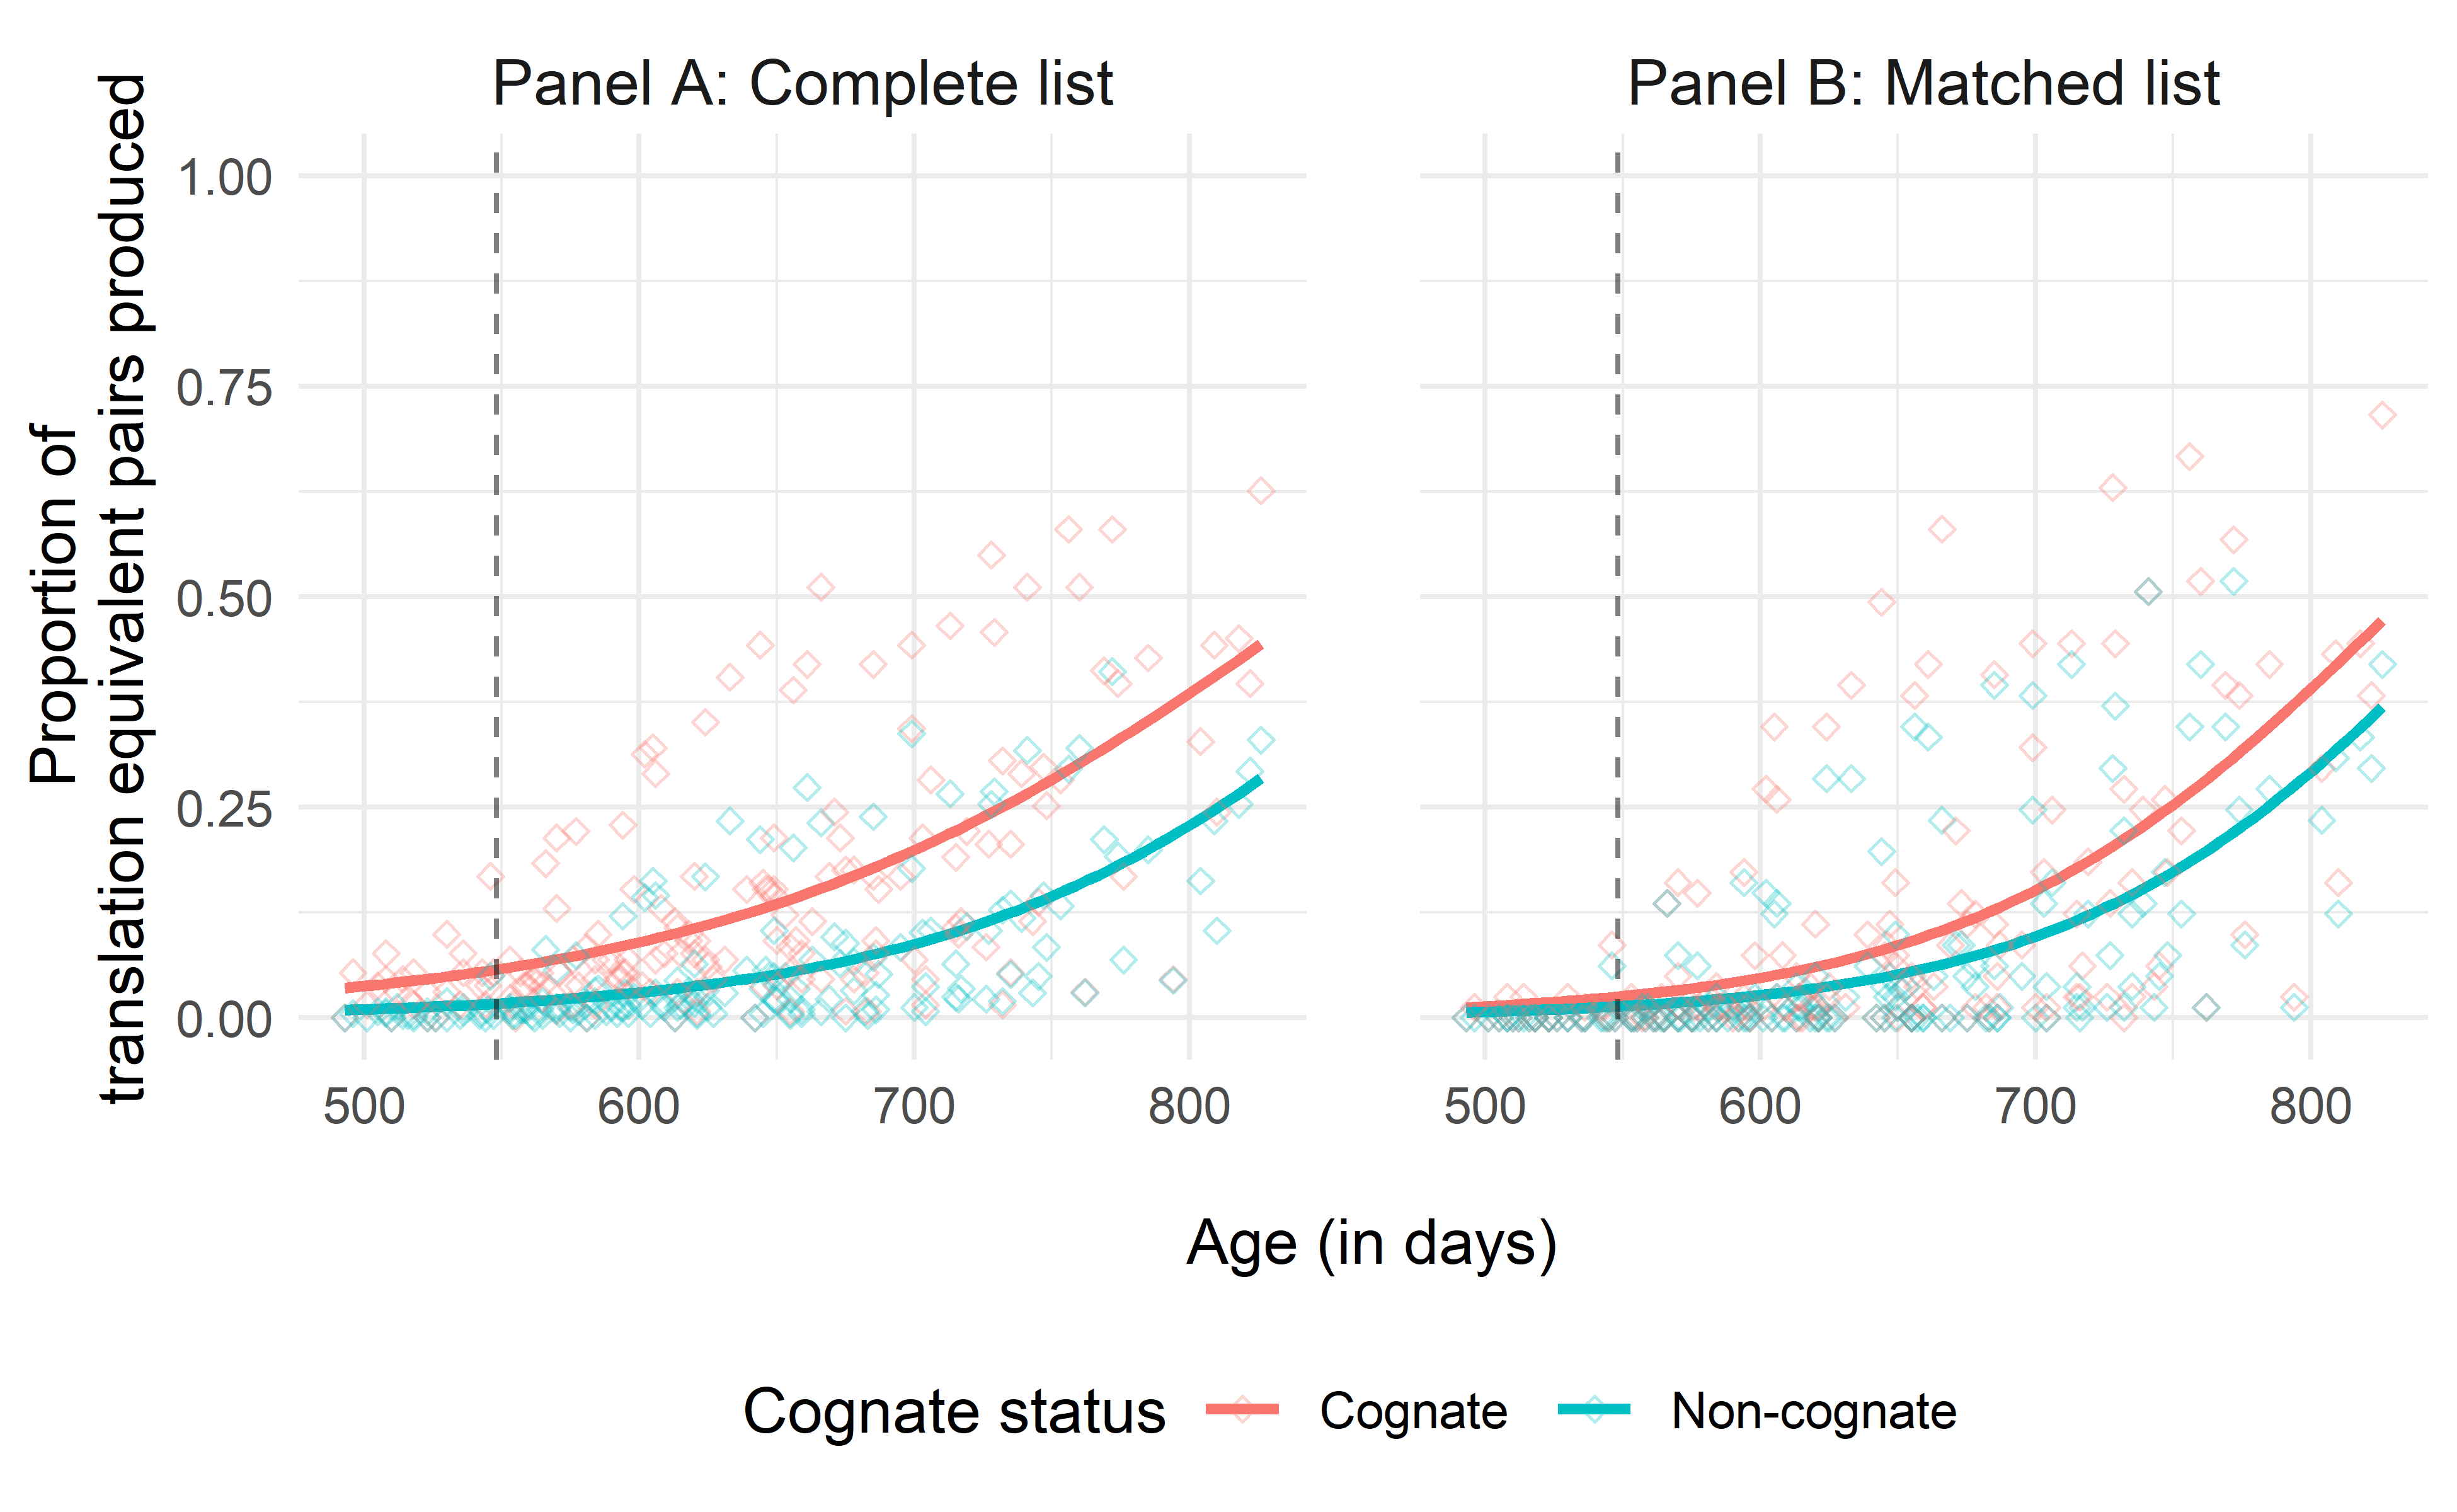
\includegraphics[width=1.2\linewidth]{CogVocab_supplemental_files/figure-latex/FigS2-1} 

}

\caption{Proportion of translation equivalent pairs produced by age and cognate status, with Panel A representing the complete list and Panel B representing the matched list. Note that the black dashed line represents the mean age of 548.3 days which serves as the reference level for age in our models.}\label{fig:FigS2}
\end{figure}

\hypertarget{summary-of-analyses}{%
\subsection{Summary of Analyses}\label{summary-of-analyses}}

Overall, the result patterns observed here with the more stringent language exposure criterion were consistent with those reported in the main analysis. This suggests that the cognate effect we observed was robust across different language exposure inclusion criteria.


\end{document}
